\documentclass[12pt]{article}
\usepackage{indentfirst}
\usepackage{graphicx}
\usepackage{textcomp}
\usepackage{siunitx}
\usepackage{subcaption}
\usepackage{amsmath}
\usepackage{setspace}
\usepackage{url}
\usepackage[a4paper,margin=2.54cm]{geometry}

\title{Computer Science II \\Project 1: Hanoi Tower}
\author{TAERAKUL Janat, \#19B60096}
\date{December 25, 2019}
\renewcommand{\UrlFont}{\small\tt}

\begin{document}

% \onehalfspacing
% \doublespacing

\maketitle

\section{Hanoi Tower}\label{sec:instr}

	The "Tower of Hanoi" is a mathematical puzzle consists of disks with different sizes and three rods as shown in figure \ref{fig:hanoi}. The objective of the game is to move the tower of disks from one rod to another. There are several rules that must be followed when moving disks:
	\begin{itemize}
	    \item Only one disk can be moved at a time.
	    \item A disk can only be placed on top of a disk larger than itself.
	\end{itemize}

	\begin{figure}[ht]
		\centering
		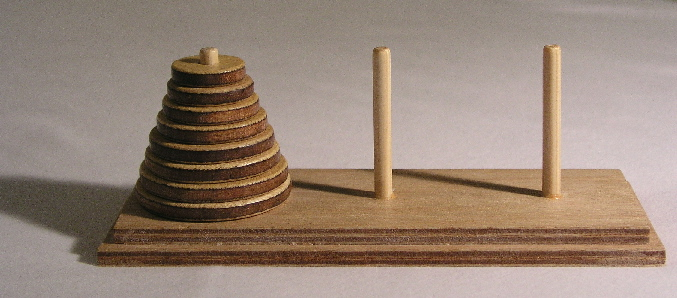
\includegraphics[height=5cm]{Hanoi.jpeg}
		\caption{The Tower of Hanoi}
		\label{fig:hanoi}
	\end{figure}

	This program (\texttt{hanoi.py}) takes an integer \texttt{n} for the number of disks as an input and assume there is a tower of \texttt{n} disks at the peg \texttt{0}. Then, it prints  
	
	\begin{figure}[ht]
		\centering
		\begin{subfigure}{.5\textwidth}
	    	\centering
		    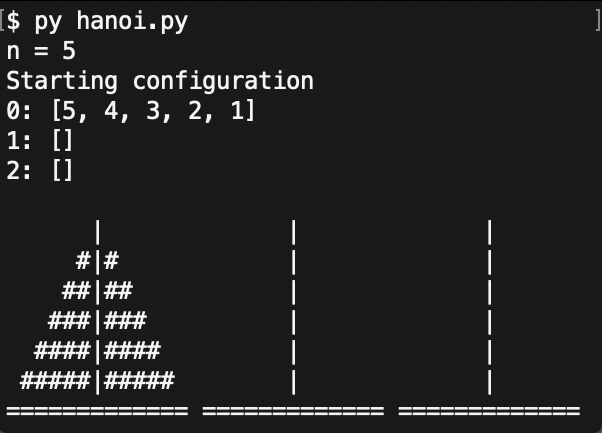
\includegraphics[height=5cm]{RunProg1.png}
		\end{subfigure}%
		\begin{subfigure}{.5\textwidth}
		    \centering
		    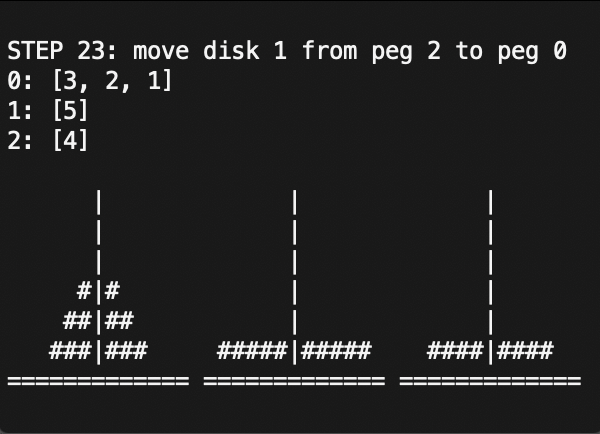
\includegraphics[height=5cm]{RunProg2.png}
		\end{subfigure}
		\caption{The display of running program}
		\label{fig:runProg}
	\end{figure}

\section{How the Program Works}\label{sec:how}

	\subsection{Global Variables}

		\begin{enumerate}
			\item \texttt{n} - Then number of disks in the tower of Hanoi.
			\item \texttt{step} - The counter for steps of moving disks. 
			\item \texttt{block} - A character for printing the disks.
		\end{enumerate}
	
	\subsection{How to Move Tower}
	
	The function \texttt{move\_tower()} is a recursive function. The base case or the smallest case for the function is when the tower is a disk. In that case, the function would just simply moves the disk by calling function \texttt{move\_disk()} to move the disk from source peg to destination peg. For the recursive part, the function considers the tower of \texttt{nb\_disk} disks as a tower of \texttt{nb\_disks-1} disks and a disk of size \texttt{nb\_disks} 
	
	\begin{verbatim}
    def move_tower(pegs, nb_disk, source, dest):
        spare = 3 - source - dest
        if nb_disk == 1:
            move_disk(pegs, source, dest)
        else:
            move_tower(pegs, nb_disk - 1, source, spare)
            move_disk(pegs, source, dest)
            move_tower(pegs, nb_disk - 1, spare, dest)
	\end{verbatim}

\section{Display Improvement}
    In the template code, there was no step numerating, so I created a global variable named \texttt{step} and used is as a step counter. I added two lines of codes and changed printing format in the \texttt{move\_disk()} function as shown in code below.
    
    \begin{verbatim}
global step
step += 1
print(f"STEP {step}: move disk {disk} from peg {source} to peg {dest}")
    \end{verbatim}

	\textbf{display\_tower(pegs)} - Input data of \texttt{pegs} into this function, the it prints the display of towers as shown in figure \ref{fig:runProg}.
	
	In addition to the example, lists-printing, display, I added the illustration of the three pegs and disks by using similar principal to the Project 1 of Computer Science course. I used loops and simple calculation for printing the game's configuration.
	
	In detail, there is a loop running through each line of the figure and another loop, nested inside, running through the three pegs. For each line of each peg, it will find if there is a disk to be printed or not. If there is a no disk to be printed, the value of \texttt{size}, which denotes the size of the disk, will be 0. If there is a disk to be printed, the value of \texttt{size} will be the size of the disk.
	
	After the program knows the size of the disk that has to be printed, it will print the disk out by printing \textit{n-size+1} spaces (the width of the pegs is one block bigger than the biggest disk) and \texttt{size} blocks. Then, the program prints a pole (\texttt{|}) follows with \texttt{size} blocks and \textit{n-size+2} spaces (add one space for a space between pegs).
	
	Lastly, the program prints (\texttt{=}) as the bases of the pegs by simply loops three times for three pegs and prints \texttt{2*n+3} times of \texttt{=} for each time.

	\begin{verbatim}
		def display_tower(pegs):
		    for height in range(n + 1, 0, -1):
		        for peg in pegs:
		            if height <= len(peg):
		                size = peg[height-1]
		            else:
		                size = 0

		            for k in range(n - size + 1):
		                print(' ', end = '')
		            for k in range(size):
		                print(block, end = '')
		            print('|', end = '')
		            for k in range(size):
		                print(block, end = '')
		            for k in range(n - size + 2):
		                print(' ', end = '')
		        print()

		    for i in range(3):
		        for j in range(2 * n + 3):
		            print('=', end = '')
		        print(' ', end = '')

		    print()
		    print()
	\end{verbatim}

	


\end{document}